\documentclass[a4paper,10pt]{article}

\usepackage{graphicx}
\usepackage{amsmath}
\usepackage[latin1]{inputenc}
\usepackage[spanish]{babel}

\title{ \textbf{ 6620. Organizaci\'on de Computadoras\\
Trabajo Pr\'actico 0: \\
Infraestructura B\'asica}}

\author{	Gonz\'alez, Juan Manuel, \textit{Padr\'on Nro. 79.979} \\
            	\texttt{ juan0511@yahoo.com } \\[2.5ex]
            	Arg\"uello, Osiris, \textit{Padr\'on Nro. 83.062} \\
            	\texttt{ osirisarguello@yahoo.com.ar } \\[2.5ex]
		Paez, Ezequiel Alejandro, \textit{Padr\'on Nro. 84.474} \\
		\texttt{ skiel85@gmail.com } \\[2.5ex]
            	\normalsize{1er. Cuatrimestre de 2012} \\
            	\normalsize{66.20 Organizaci\'on de Computadoras  $-$ Pr\'atica Jueves} \\
            	\normalsize{Facultad de Ingenier\'ia, Universidad de Buenos Aires} \\
       }

\date{}

\begin{document}
\maketitle
\thispagestyle{empty}  % quita el nmero en la primer pagina


\begin{abstract}
El presente trabajo tiene como objetivo familiarizarse con las herramientas de software que ser\'an usadas en los siguientes trabajos, implementando un programa (y su correspondiente documentaci\'on) que resuelva el problema piloto planteado, una implementaci\'on de los algoritmos de ordenamiento \textit{Mergesort} y \textit{Selectionsort} en lenguaje C. A su vez, se utilizar\'a el programa GXemul para simular un entorno de desarrollo en una m\'aquina MIPS, a fin de obtener el c\'odigo en Assembly MIPS32 de la implementaci\'on realizada. Finalmente, procederemos a realizar mediciones para evaluar las posibilidades de mejora y el desempe\~no relativo entre ambos algorimos, utilizando los programas \textit{time} y \textit{gprof}.


\end{abstract}

\pagebreak

\setcounter{page}{2}
\section{Introducci\'on}
Al comenzar a utilizar nuevas herramientas, en cualquier \'ambito, es necesaria una breve introducci\'on al funcionamiento de las mismas: tener una noci\'on de las prestaciones que ofrecen, asi tambi\'en como de sus limitaciones.\\
Como primer objetivo en la materia, nos proponemos adentrarnos en el funcionamiento del emulador GXemul. Nuestra meta ser\'a emular una plataforma MIPS DECstation 5000/200 (ejecutando un sistema operativo NetBSD), para poder desde all\'i desarrollar programas en lenguaje C. Estos ser\'an compilados y ejecutados haciendo uso de la herramienta GCC (GNU Compiler Collection), mediante el cual tambi\'en ser\'a posible obtener, a posteriori, el c\'odigo MIPS32 del programa.\\
Una vez cumplido este objetivo, experimentaremos con los programas \textit{time} y \textit{gprof}, a fin de evaluar las posibilidades de mejora y el desempe\~no relativo entre ambas implementaciones.\\
Como \'ultimo punto, aprenderemos los rudimientos de \LaTeX{} para generar la documentaci\'on relevante al trabajo pr\'actico.

\section{Programa a implementar}
El problema a resolver consiste en un implementar programa que realice ordenamiento o \textit{sorting} utilizando los algorimos de \textit{mergesort} o \textit{selectionsort}, seg\'un elija el usuario.\\

El programa debe leer los datos de entrada desde \textit{stdin} o bien desde uno o m\'as archivos. La salida del programa debe imprimirse por \textit{stdout}, mientras que los errores deben imprimirse por \textit{stderr}. El algoritmo de ordenamiento puede seleccionarse mediante las opciones \textbf{-m} o \textbf{-s} para \textit{mergesort} o \textit{selectionsort} respectivamente.

\section{Consideraciones sobre el desarrollo}
A continuaci\'on se detallan las consideraciones tenidas en cuenta para el desarrollo del trabajo pr\'actico. Hemos decidido separar las que surgen del Dise\~no de las que surgen en la implementaci\'on.

\subsection{Consideraciones de Dise\~no}

El programa a desarrollar consta a grandes rasgos de un parser encargado de leer los par\'ametros de entrada, y las funciones que realizan la lectura de los archivos y las funciones encargadas de realizar el ordenamiento mediante los algoritmos solicitados. Dada la complejidad y extensi\'on de algunas de las funciones desarrolladas, se decidi\'o separar el programa en una serie de archivos, a modo de mejorar su legibilidad y organizaci\'on. A continuaci\'on se presenta la lista de archivos que componen el proyecto:\\
\\
\begin{tabular}{|l|l|}
\hline
Archivo & Descripci\'on \\ \hline
tp0.c & Funci\'on main e int\'erprete de l\'inea de comandos. \\
manejoes.h & Encabezado correspondiente a 'manejoes.c'. \\
manejoes.c & Parser de entrada y funci\'on de escritura de salida. \\
sort.h & Encabezado correspondiente a 'sort.c'. \\
sort.c & Implementaci\'on de \textit{mergesort} y \textit{selectionsort}. \\
deferrores.h & Definici\'on de los c\'odigos de error internos del programa. \\
\hline
\end{tabular}\\
\\\\

El dise\~no de la aplicaci\'on se realiz\'o pensando en varias <<capas>>. Una capa es encargada de analizar y validar opciones de ejecuci\'on, otra capa, la encargada de realizar las operaciones principales de conversi\'on y otras m\'as peque\~nas encargadas de emitir mensajes de error o informaci\'on de ayuda en pantalla para el usuario.\\

Dado que la aplicaci\'on puede tomar par\'ametros variables de ejecuci\'on o adoptar valores por defecto, se realiz\'o un an\'alisis completo de todas las opciones que un usuario puede ingresar, aceptando aquellas que fueren v\'alidas y rechazando las que no, con el consiguiente mensaje de error que el usuario visualizar\'a en pantalla. En caso de no ser especificado un algoritmo de ordenamiento, el programa asumir\'a la opci\'on \textbf{-m}, correspondiente a \textit{mergesort}.\\

La aplicaci\'on fue implementada en lenguaje ANSI C, es decir que est\'a garantizada la compilaci\'on exitosa ante la utilizaci\'on de la opci\'on \textit{-ansi} en GCC.\\

La siguiente capa importante, es la correspondiente a los algoritmos de ordenamiento. Se desarrollaron dos algoritmos de ordenamiento: \textit{mergesort} y \textit{selectionsort}. La implementaci\'on para ambos algoritmos b\'asicamente consta de procesos similares, ligeramente diferenciados en el punto en que se invoca una funci\'on ANSI C distinta de acuerdo al tipo de ordenamiento que se est\'e realizando.\\

A grandes rasgos, la soluci\'on intenta leer el \textit{stream} de entrada de datos que es especificado por el usuario. Puede constar de varios archivos o directamente ser la entrada est\'andar. De no resultar satisfactoria esta operaci\'on, ya sea porque el archivo no existe o se produjere un fallo en el disco en el momento de la lectura, se retorna de inmediato el correspondiente c\'odigo de error. Si pueden tomarse los datos de entrada, el programa procede a su almacenamiento, si se trata de varios archivos estos son concatenados. Para resolver el almacenamiento de los datos se dise\~n\'o un tipo de dato especial, que consta de un char* y dos variables de control, a fin de ir reservando memoria en forma d\'inamica, a medida que es requerida. Como \'ultimo paso, una vez que se cuenta con los datos cargados, se continua la ejecuci\'on realizando el ordenamiento indicado por el usuario, volcando el resultado de dicha operaci\'on por la salida est\'andar o \textit{stdout}. Dado que el programa debe funcionar con archivos binarios, las lecturas y escrituras se realizan mediante las funciones \textit{fread} y \textit{fwrite}.\\

Por otro lado, se dise\~n\'o el programa de modo que todas las salidas por \textit{stdout} o \textit{stderr} se encuentren en la funci\'on main o en funciones dedicadas a ese prop\'osito. En el caso del mensaje de ayuda y el de versi\'on del programa, se codificaron dos funciones espec\'ificas, mientras que los mensajes de error son mostrados justo antes de finalizar la ejecuci\'on del programa, en la funci\'on main. Para lograr esto, se definieron c\'odigos de error internos al programa que son devueltos a main para su interpretaci\'on por cada una de las funciones que son llamadas. Dichos c\'odigos, definidos en el archivo 'deferrores.h', son:\\
\\
2: ERROR\_RESERVA\_INICIAL\_MEMORIA\\
3: ERROR\_RESERVA\_MEMORIA\\
4: ERROR\_ARCHIVO\_ENTRADA\\\\
La ejecuci\'on del programa se interrumpe por cualquiera de estos errores, mostrando al usuario un mensaje afin. Los c\'odigos 0 y 1 son utilizados para la devoluci\'on al SO del resultado de la ejecuci\'on, siendo:\\
\\
0: Ejecuci\'on sin problemas.\\
1: Error de ejecuci\'on.\\
\\
El procesamiento e interpretaci\'on de los comandos ingresados desde la consola es manejado mediante la biblioteca 'getopt', evitando as\'i la implementaci\'on de un parser para este fin. Dado que el enunciado presenta un mensaje de ayuda en idioma ingl\'es, se han codificado todas las salidas en este idioma. Asimismo, los mensajes de error fueron formateados para imitar la salida de 'getopt', con el fin de presentar los errores en forma consistente.\\
\\
Finalmente, cabe destacar que todas las impresiones del programa son ruteadas por \textit{stdout}, y los mensajes de error a trav\'es de \textit{stderr}.\\
\\
\subsection{Consideraciones de Implementaci\'on}

Cabe destacar que para implementar el trabajo pr\'actico se parti\'o de la totalidad del programa implementado en lenguage C (se ha respetado el est\'andar ANSI) y luego se procedi\'o a traducir a assembly de MIPS el c\'odigo final, con el uso de GCC.

\subsubsection{Portabilidad de la soluci\'on}
El programa est\'a dise\~nado para poder ser ejecutado en diferentes plataformas, como por ejemplo NetBSD (PMAX) y la versi\'on de Linux usada para correr el simulador, GNU/Linux (i686). El haber codificado el proyecto en lenguaje ANSI C garantiza que pueda ser compilado en ambas plataformas sin problemas, dotando al programa de un grado m\'inimo de portabilidad.\\
Por otro lado, se destaca que se entrega junto con el presente informe dos versiones del c\'odigo fuente, una en formato C y la otra en c\'odigo assembly MIPS.\\

Las principales funciones y estructuras en nuestra implementaci\'on son las siguientes:

\subsubsection{Cadena de bytes \textit{tDynArray}}
Para implementar la cadena de bytes que utiliza el programa desarrollado (\textit{tDynArray}), se ha utilizado un arreglo en memoria din\'amica, que crece reservando memoria autom\'aticamente al agrandarse la cadena cuando es necesario.

\subsubsection{procesarEntrdada}
Esta funci\'on se encarga de tomar los archivos de entrada (o \textit{stdin} seg\'un corresponda), abrirlos y operar con el \textit{tDynArray} para ir guardando el contenido de todos los archivos especificados por el usuario. Los archivos se van abriendo dentro de un bucle \textit{for}, y la lectura se realiza mediante la funci\'on \textit{fread}.

\subsubsection{procesarSalida}
Esta funci\'on tiene como objetivo presentar el resultado del ordenamiento, para lo que utiliza la funci\'on \textit{fwrite}. La salida es \'unicamente por salida est\'andar o \textit{stdout}.

\subsubsection{mergeSort}
Este m\'etodo toma el array de caracteres leido de los archivo, lo divide en 2 partes e invoca recursivamente la funcion \textbf{mergeSort} sobre cada parte. Como ultimo paso fusiona ambas partes, ordenandolas.

\subsubsection{selectionSort}
Este m\'etodo recorre el array de caracteres, buscando el menor caracter en cada iteraci\'on y ubic\'andolo al principio del array.\\

\section{Generaci\'on de ejecutables y c\'odigo assembly}
Para generar el ejecutable del programa, debe correrse la siguiente sentencia en una terminal:
\begin{verbatim}
$ gcc -Wall -o tp0 tp0.c manejoes.c sort.c
\end{verbatim}

Para generar el c\'odigo MIPS32, debe ejecutarse lo siguiente:
\begin{verbatim}
$ gcc -Wall -S -mrnames tp0.c manejoes.c sort.c
\end{verbatim}

N\'otese que para ambos casos se han activado todos los mensajes de 'Warning' (-Wall). Adem\'as, para el caso de MIPS, se han habilitado otras dos banderas: '-S' que detiene al compilador luego de generar el assembly y '-mrnames' que tiene como objetivo generar la salida utilizando los nombres de los registros en vez de los n\'umeros de registros.
\pagebreak

\section{Corridas de prueba}

En esta secci\'on se presentan algunas de las distintas corridas que se realizaron para probar el funcionamiento del trabajo pr\'actico.\\
\\
En primer lugar se mostr\'o el mensaje de ayuda, y luego se imprimi\'o la versi\'on del programa:
\begin{center}
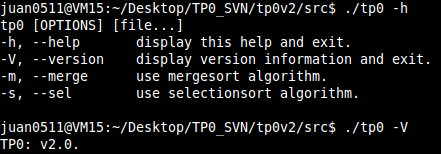
\includegraphics[scale=0.60]{1.png}
\end{center}

Luego, se ejecut\'o la prueba provista por la c\'atedra en el enunciado del trabajo pr\'actico:
\begin{center}
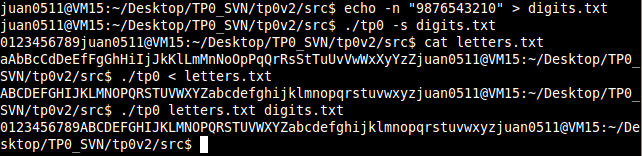
\includegraphics[scale=0.60]{2.png}
\end{center}

\begin{center}
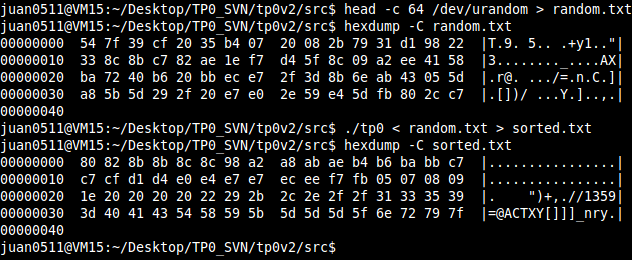
\includegraphics[scale=0.60]{3.png}
\end{center}
\pagebreak

Finalmente, se presenta un ejemplo m\'as mostrando alguna de las salidas posibles, obtenida para casos en los trabaja con archivos binarios y cuando se intenta abrir un archivo inexistente:\\
\begin{center}
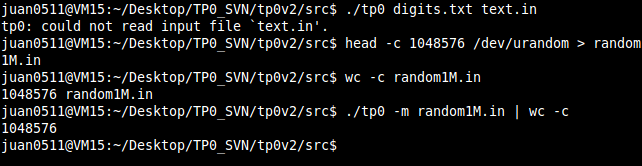
\includegraphics[scale=0.60]{4.png}
\end{center}
\pagebreak

\section{Mediciones} 
Se compar\'o la performance de cada uno de los algoritmos realizando pruebas con el comando time. Se tom\'o el tiempo insumido por cada uno de los algoritmos tomando archivos de diferentes tama\~nos y de diferente aleatoridad (completamente aleatorio, aleatorio ordenado y aleatorio inversamente ordenado).

Los archivos completamente aleatorios fueron generados leyendo bytes de /dev/urandom de un sistema linux. Los archivos de prueba aleatorios ordenados se generaron ordenando los archivos anteriores con el propio programa desarrollado. Y los archivos inversamente ordenados fueron generados invirtiendo estos \'ultimos archivos con un simple algoritmo hecho en C.

Se realizaron gr\'aficos comparativos para cada una de las situaciones con curvas que representan a cada algoritmo, representando el tiempo insumido (milisegundos) en relaci\'on con el tama\~no del archivo de entrada.

Este gr\'afico representa los dos m\'etodos para el caso de un \textit{array} ya ordenado:
\begin{center}
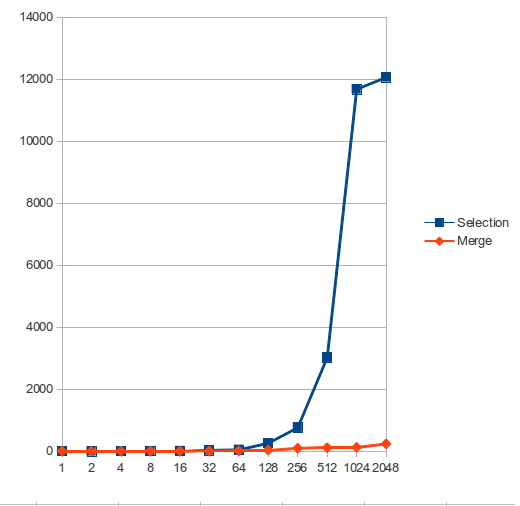
\includegraphics[scale=0.50]{sorted.png}
\end{center}

Este gr\'afico representa los dos m\'etodos para el caso de un \textit{array} en orden inverso:
\begin{center}
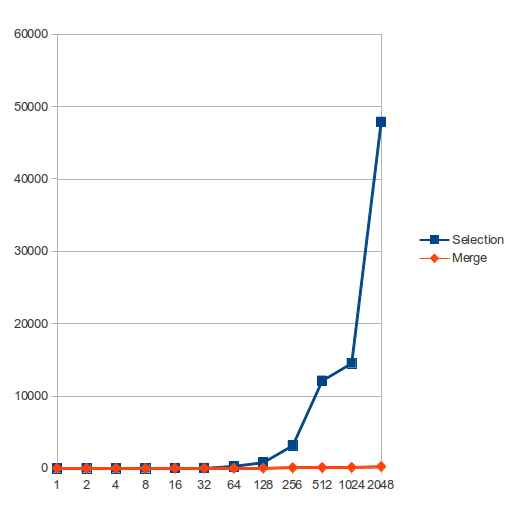
\includegraphics[scale=0.50]{reverted.png}
\end{center}

Este gr\'afico representa los dos m\'etodos para el caso del promedio de diez \textit{arrays} con datos tomados al azar:
\begin{center}
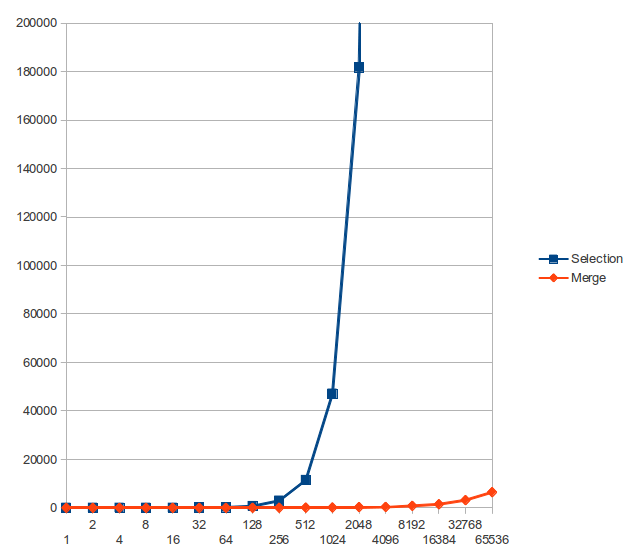
\includegraphics[scale=0.50]{random.png}
\end{center}

Observamos en estos gr\'aficos como la curva de crecimiento del tiempo insumido del \textit{selectionsort} es casi exponencial, mientras que la curva del \textit{mergesort} es mucho m\'as estable.

Tambi\'en se presenta un gr\'afico que muestra el speedup de la mejora de pasar de \textit{selectionsort} a \textit{mergesort} para cada una de las tres situaciones. Observamos en este gr\'afico que la mejora es muy grande para arreglos de gran tama\~no, pero para arreglos peque\~nos casi no hay diferencia:
\begin{center}
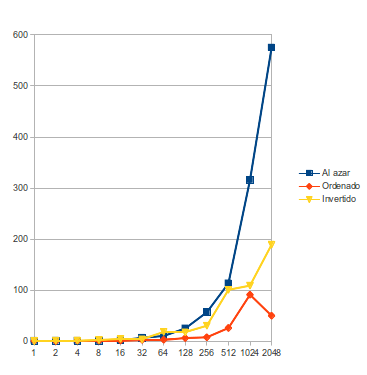
\includegraphics[scale=0.50]{speedup-time.png}
\end{center}
\pagebreak

\section{Profiling} 
Con el objetivo de proponer una mejora en la implementaci\'on realizada, se utiliz\'o el programa \textit{gprof} para obtener la distribuci\'on de tiempos durante la ejecuci\'on de la aplicaci\'on. Se presentan dos tablas con los resultados m\'as significativos, para cada algoritmo de ordenamiento:

\subsection{Mergesort}

\begin{tabular}{|l|l|l|l|l|l|l|}
\hline
percent & cumulative seconds & self seconds & calls & self s/call & total s/call & name \\ \hline
 96.74   &   3.26  &   3.26   &     1  &   3.26  &   3.26  & mergeSort \\
  3.26   &   3.37  &   0.11   &     1  &   0.11  &   0.11  & procesarEntrada \\
  0.00   &   3.37  &   0.00   &     1  &   0.00  &   0.00  & imprimirSalida \\
\hline
\end{tabular}\\

Utilizo un archivo con 6553600 bytes para que el procesamiento dure tiempo suficiente para notar las diferencias de tiempo entre cada m\'etodo y minimizar el impacto del tiempo de lectura de disco.

En esta prueba el tiempo total insumido fue de 3,37 segundos.

La mayor parte del tiempo se la lleva la ejecuci\'on del m\'etodo merge con un 97\% del tiempo (3,26 segundos), y por eso es el que conviene optimizar. Si este m\'etodo fuera optimizado al punto de costar un tiempo despreciable, el tiempo total del programa ser\'ia de 0,11 segundos, entonces el speedup máximo ser\'ia de 3,37/0,11 = 30,6.\\

\subsection{Selectionsort}
La distribuci\'on de tiempos para este algoritmo es:

\begin{tabular}{|l|l|l|l|l|l|l|}
\hline
percent & cumulative seconds & self seconds & calls & self s/call & total s/call & name \\ \hline
100.00  &  268.50  & 268.50  &      1  & 268.50  & 268.50 & selectionSort \\
  0.00  &  268.50  &   0.00  & 203999  &   0.00  &   0.00 & swap \\
  0.00  &  268.50  &   0.00  &      1  &   0.00  &   0.00 & imprimirSalida \\
  0.00  &  268.50  &   0.00  &      1  &   0.00  &   0.00 & procesarEntrada \\
\hline
\end{tabular}\\

Fue analizado con un archivo de 204800 bytes por las mismas razones que elegimos el archivo del mergeSort. Pero en este caso es un archivo m\'as peque\~no porque el selectionSort es m\'as lento. El m\'etodo selectionSort es el que conviene optimizar, ya que es el que se lleva casi el 100\% del tiempo. Si este m\'etodo se optimizara al punto de ser despreciable el tiempo que consume, el speedup m\'aximo tender\'ia a infinito.
\pagebreak

\section{C\'odigo fuente C y MIPS32} 
Tanto el c\'odigo C como el c\'odigo MIPS32 que fue generado en el trabajo pr\'actico ha sido incluido en el CD entregado junto al presente informe.
\pagebreak

\section{Conclusiones}
El trabajo pr\'activo motivo de este informe ha presentado al equipo diversos desaf\'ios. En primer lugar cabe mencionar la adaptaci\'on a un ambiente basado en GNU/Linux, no dominado por todos sus integrantes en igual manera. Tambi\'en es destacable la dificultad inicial que trajo la correcta configuraci\'on del ambiente virtual utilizado para emular la m\'aquina MIPS, aunque esto fue paliado en gran parte por la documentaci\'on y explicaciones provistas por la c\'atedra. Finalmente, tambi\'en fue invertida una cantidad considerable de tiempo en aprender a utilizar e investigar sobre \LaTeX{}, ya que si bien permite obtener muy buenos resultados, se requiere de mucha lectura para poder aprovechar todo su potencial. En este sentido, el modelo de informe suministrado tambi\'en fue muy util para dar los primeros pasos.\\
A su vez, hemos comprobado la utilidad de utilizar la ley de Amdahl para comparar la performance de algoritmos, y su utilidad para comprender como realizar optimizaciones de los mismos, utilizada en conjunto con utilidades como \textit{time} y \textit{gprof}.\\
La ley de Amdahl en este caso no es de mucha ayuda porque los algoritmos implementados constan de una sola funci\'on y es obvio que todo el peso recae sobre la funci\'on de ordenamiento. Pero en algoritmos m\'as complicados con m\'as funciones, el profiling nos puede ayudar a determinar cual funci\'on es la m\'as pesada y entonces si poner todo el esfuerzo en optimizarla.\\
Por las razones expuestas, consideramos muy necesario un trabajo pr\'actico introductorio de esta naturaleza, sin gran dificultad algor\'itmica o te\'orica pero justamente orientado a nivelar e introducir los elementos a utilizar en las dem\'as actividades pr\'acticas que se desarrollar\'an en el curso.\\
Como conclusi\'on final, podemos considerar que hemos logrado obtener un buen manejo de las herramientas introducidas en este primer proyecto.

\pagebreak

\begin{thebibliography}{99}
	

\bibitem{MS} Merge-sort, http://en.wikipedia.org/wiki/Merge\_sort

\bibitem{SS} Selection-sort, http://en.wikipedia.org/wiki/Selection\_sort

\bibitem{TIME} \textit{time} man page, http://unixhelp.ed.ac.uk/CGI/man-cgi?time

\bibitem {GPROF} GNU \textit{gprof}, http://www.cs.utah.edu/dept/old/texinfo/as/gprof.html

\bibitem{GXEMUL} GXemul, http://gxemul.sourceforge.net/

\bibitem{NETBSD} The NetBSD Project, http://www.netbsd.org/

\bibitem{LIBROC} Kernighan, Brian W. / Ritchie, Dennis M. \underline{El Lenguaje De Prorgamaci\'on C}. Segunda Edici\'on, PRENTICE-HALL HISPANOAMERICANA SA, 1991.

\bibitem{LATEX} Oetiker, Tobias, "The Not So Short Introduction To LaTeX2", http://www.physics.udel.edu/$\sim$dubois/lshort2e/

\end{thebibliography}

\end{document}
